%
% buchberger.tex
%
% (c) 2026 Nathanael Fässler, OST Ostschweizer Fachhochschule
%
% !TEX root = ../../buch.tex
% !TEX encoding = UTF-8
%
\section{Polynomielle Gleichungssysteme
\label{buchberger:section:buchberger}}
\kopfrechts{Polynomielle Gleichungssysteme}
Das Gleichungssystem
\begin{equation}
  \begin{cases}
  x^2 -y = 0 \\
  x + y^2 = 3
  \end{cases}
  \label{buchberger:polynom-gleichungssystem-1}
\end{equation}
lässt sich nicht mehr mit dem Gauss-Algorithmus lösen.
Der Grund ist, dass es Variablen mit Potenzen $> 1$ beinhaltet, also nicht linear.

Um solche nonlineare multivariate\footnote{Multivariat bedeutet, dass mehrere Variablen vorkommen.} Gleichungssysteme zu lösen eignet sich der Buchberger-Algorithmus.
Ein Gleichungssystem wie
\begin{equation}
  \begin{cases}
  5xy + 2y^3 +  5y^8z + z^3 = 100 \\
  3x^2y^4z^9 + 2z^2 = 1 \\
  (x-1)\,(y-2)\,(z-3) = 0 \\
  \end{cases}
  \label{buchberger:polynom-gleichungssystem-2}
\end{equation}
lässt sich damit auch lösen.

Terme mit mehreren Variablen wie $5xy$ sind hier im Gegensatz zu linearen Gleichungen erlaubt.
Die Klammern der letzten Gleichung stellen kein neues Problem dar, da sie beim ausmultiplizieren auch in die bekannte Koeffizientenform gebracht werden können.


\subsection{Geschichte}
\label{buchberger:subsection:geschichte}
Im Jahre 1965 hat der österreichische Mathematik-Student Bruno Buchberger in seiner Dissertation die Gröbner-Basis entwickelt.
Er hat sie nach seinem Professor Wolfgang Gröbner benannt.
Zu seiner Dissertation gehörte auch der Buchberger-Algorithmus mit dem man Gröbner-Basen berechnen kann.
Der Algorithmus wurde zu einem wichtigen Bestandteil von Computeralgebrasystemen.

\subsection{Buchberger-Algorithmus}
\label{buchberger:subsection:buchberger-algorithmus}

\begin{algorithm}
\caption{Pseudo-Code des Buchberger-Algorithmus in C++/Java ähnlichem Style
\label{buchberger:pseudo-code}}
\begin{algorithmic}[1]
  \State \textbf{function} Buchberger(Menge$<$Polynom$>$ startPolynome) \{
    \State \quad Menge$<$Polynom$>$ basis = startPolynome;
    \State \quad Menge$<$Polynom$>$ alteBasis = \{\};
    \State \quad \textbf{while} (basis $\neq$ alteBasis) \{
      \State \quad \quad alteBasis = basis;
      \State \quad \quad \textbf{for} (Pair$<$Polynom$>$ (p, q) $\in$ alteBasis) \{
        \State \quad \quad \quad Polynom rest = spezialDivision((p, q), alteBasis);
        \State \quad \quad \quad \textbf{if} (rest $\neq$ 0) \{
          \State \quad \quad \quad \quad basis = basis $\cup$ \{rest\}; \Comment{Fügt neues Polynom zur Basis hinzu.}
        \State \quad \quad \quad \} % end if
      \State \quad \quad \} % end for
    \State \quad \} % end while
    \State \quad \textbf{return} basis;
  \State \} % end function
\end{algorithmic}
\end{algorithm}

Dieses Kapitel soll dem Leser eine Idee geben wie der Buchberger-Algorithmus funktioniert und wie man ihn anwendet.
Wie der Algorithmus genau funktioniert erklärt Lamagna in seinem Buch~\cite{buchberger:computer-algebra} in Kapitel 8.%cite{buchberger:computer-algebra}

Wie beim Gauss-Algorithmus müssen die Gleichungen zunächst in eine geeignete Form gebracht werden.
Die Gleichungen werden in Polynome umgewandelt, wobei sie vorher auf die Form $p(x) = 0$ umgestellt werden.
Das Gleichungssystem
\begin{equation}
  \begin{cases}
  x^2 -y = 0 \\
  x + y^2 -3 = 0
  \end{cases}
  \label{buchberger:polynom-gleichungssystem-3}
\end{equation}
wird in die Menge der Polynome 
\begin{equation}
  B
  =
  \{
    x^2 -y,
    x + y^2 - 3
  \}
  \label{buchberger:polynom-gleichungssystem-4}
\end{equation}
umgeformt.

Dabei ist wichtig, dass alle Polynome eine eindeutige Ordnung der Terme besitzen.
Zum Beispiel legt die lexikographische Ordnung fest, dass zuerst alle Terme mit dem höchsten Grad bezüglich $x$ stehen.
Wenn dies auf mehrere Terme zutrifft, wird innerhalb dieser Gruppe bezüglich des Grads von $y$ sortiert und dann bezüglich $z$ und so weiter bis zur letzen Variable.
Dies ist nötig, da der Buchberger-Algorithmus eine spezielle Variante der Polynomdivision verwendet, wobei der leitende Term bekannt sein muss.

Der Pseudo-Code des Algorithmus~\ref{buchberger:pseudo-code} zeigt vereinfacht den Ablauf auf.
Die Funktion spezialDivision ist in sich selbst ein komplizierter Algorithmus und wird im folgenden nur grob erklärt.
s
Der Algorithmus startet mit einer Menge von Polynomen, welche die Basis genannt wird (Zeile 2).
Aus den Polynomen der Basis werden alle möglichen Paare gebildet (Zeile 4).
Mit einer speziellen Polynomdivision\footnote{Im Pseudo-Code wird die Funktion spezialDivision genannt.}(Zeile 7), die jeweils eines der Paare als Dividend und die ganze Basis als Divisor einbezieht, wird ein Quotient mit Rest berechnet.
Dabei will der Algorithmus herausfinden ob jeweils zwei Polynome als Paar eine Information tragen, die in der Basis noch nicht enthalten ist.
Darum ist auch in einer dieser Polynomdivision-Operationen immer ein Paar und die ganze Basis beteiligt.

Die neue Information die bei dieser Polynomdivision gewonnen wurde ist der Rest der Division.
Dieser Rest wird als Polynom zur Basis hinzugefügt um somit die neu gewonnene Information zu behalten (Zeile 9).
Durch die Vergrösserung der Basis haben sich auch neue Polynom-Paare ergeben.
Diese neuen Paare werden auch den Polynomdivisions-Schritt durchlaufen.

Wenn ein Paar keine neuen Informationen liefert, zeigt sich das daran, dass das Paar durch die Basis teilbar ist ohne Rest.
Also wenn der Rest $0$ ist, war das Paar nutzlos (Zeile 8).
Die Tatsache, dass das Polynom $0$ keine Information liefert macht durchaus Sinn:
Wenn man das Polynom $0$ als Gleichung interpretiert muss man es gleich Null setzen und die Gleichung $0 = 0$ ist immer wahr, und liefert keine Information.

Die Prozedur wird solange wiederholt bis keine neuen Polynome zur Basis hinzugefügt werden können (Zeile 4).
Das Resultat ist eine Basis mit mindestens so vielen Polynome wie die ursprüngliche Basis (Zeile 13).
Der Grund ist, dass nur Polynome hinzugefügt aber nie entfernt wurden.

Im letzten Schritt, der hier nicht genauer erklärt wird, und auch nicht im Pseudo-Code~\ref{buchberger:pseudo-code} enthalten ist, werden redundante Polynome entfernt und das Ergebnis ist eine sogenannte \emph{Gröbner-Basis}.

Wenn man den Algorithmus auf das System \eqref{buchberger:polynom-gleichungssystem-1} 
anwendet erhält man die Gröbner-Basis 
\begin{equation}
  G
  =
  \{
    x^4 + x - 3,
    x^2 - y
  \}
  \label{buchberger:polynom-gleichungssystem-5}
\end{equation} 
, woraus sich das Gleichungssystem
\begin{equation}
  \begin{cases}
  x^4 + x = 3 \\
  x^2 - y = 0
  \end{cases}
  \label{buchberger:polynom-gleichungssystem-6}
\end{equation}
konstruieren lässt.

Das Gleichungssystem ist zwar noch nicht gelöst, aber es besitzt eine nützliche Eigenschaft.
Nämlich, dass die erste Gleichung nur noch die Variable $x$ beinhaltet.
Eine Gleichung mit nur einer Variable lässt sich numerisch lösen mit z.B. dem \emph{Newton-Verfahren}.
Wie beim Gauss-Algorithmus erhält man beim Buchberger-Algorithmus eine Zeilenstufenform, 
wobei sich immer das Ergebnis der vorherigen Gleichungen in die nächste einsetzen lassen.
Weil es sich hier um nonlineare Gleichungen handelt, kann eine Gleichung mehrere Lösungen für eine Variable ergeben.
Beim Rückwärtseinsetzen müssen dann alle Kombinationen der bisherigen Lösungen eingesetzt werden.



\subsection{Visualisierung eines Gleichungssystems}
\label{buchberger:subsection:visualisierung}
\begin{figure}
\centering
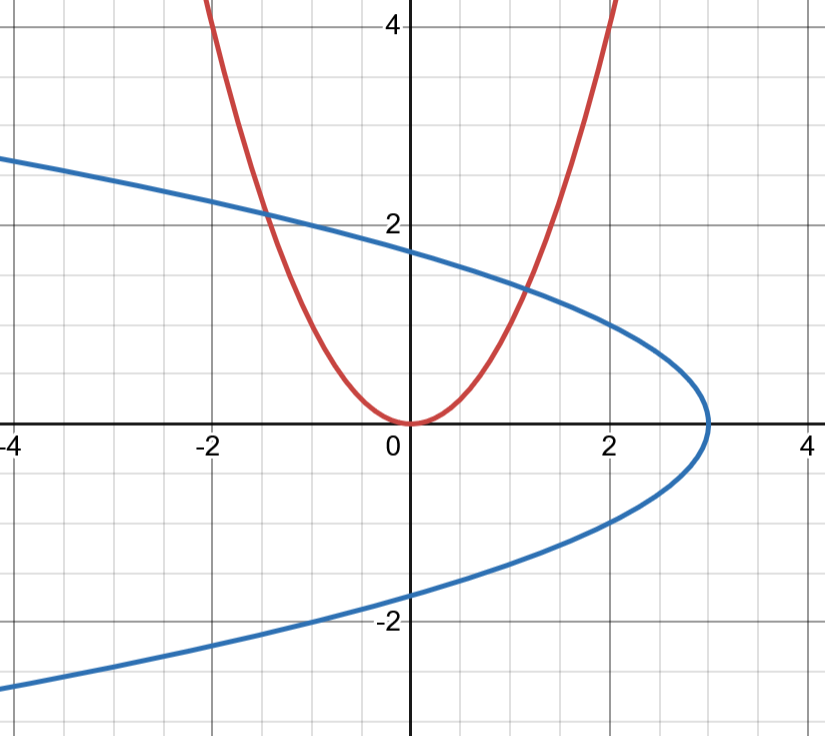
\includegraphics[width=0.7\textwidth]{papers/buchberger/images/equationSystem1.png}
\caption{Visualisierung des Gleichungssystems \protect\eqref{buchberger:polynom-gleichungssystem-1}
  \textcolor{red}{Rot: $x^2 - y = 0$},
  \textcolor{blue}{Blau: $x + y^2 = 3$}
  \label{buchberger:equationVisual1}}
\end{figure}

Der Plot~\ref{buchberger:equationVisual1}
visualisiert das Gleichungssystem \eqref{buchberger:polynom-gleichungssystem-1}
.
Alle Kombinationen von $x$ und $y$ die dazuführen, dass eine Gleichung wahr wird, sind ein Punkt auf dem roten bzw. blauen Graphen.
Die Schnittpunkte der Graphen ergeben gerade die Lösungen des Gleichungssystem.

\begin{figure}
\centering
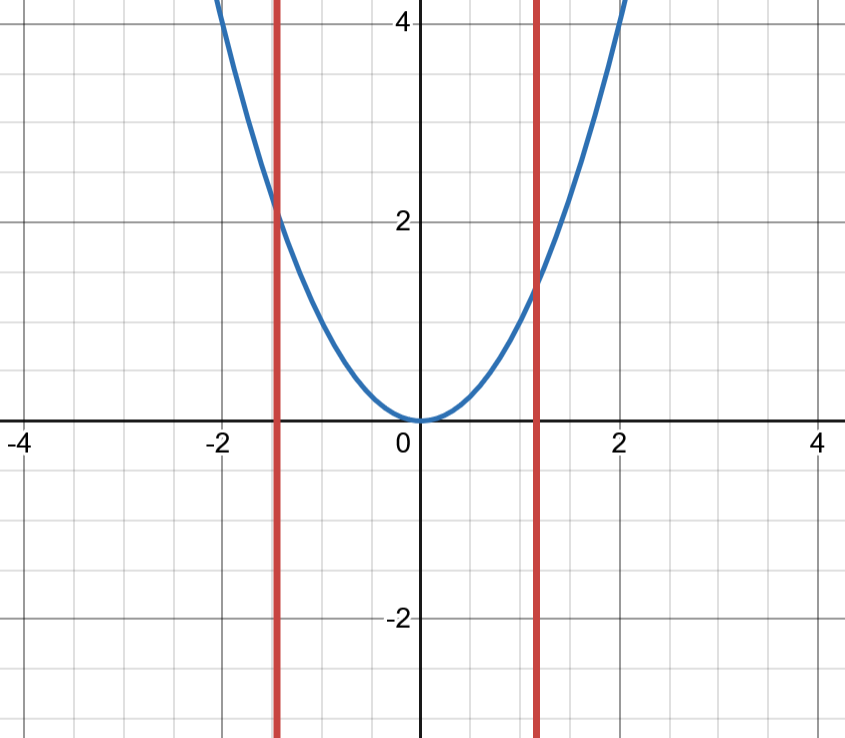
\includegraphics[width=0.7\textwidth]{papers/buchberger/images/equationSystem2.png}
\caption{Visualisierung des Gleichungssystems \protect\eqref{buchberger:polynom-gleichungssystem-6}
  \textcolor{red}{Rot: $x^4 + x = 3$},
  \textcolor{blue}{Blau: $x^2 - y = 0$}
\label{buchberger:equationVisual2}}
\end{figure}
Auf dem Plot~\ref{buchberger:equationVisual2}
ist das Gleichungssystem der Gröbner-Basis \eqref{buchberger:polynom-gleichungssystem-6}
dargestellt.
Die Eigenschaft, dass die erste Gleichung nur die Variable $x$ beinhaltet wird hier auf interessante Weise sichtbar:
Die Gleichung besteht nur noch aus vertikalen Geraden.
Das erklärt sich dadurch, dass die Gleichung nicht mehr von $y$ abhängt und somit die y-Achse nicht mehr relevant ist für die Gleichung.
Die Gleichung wurde sozusagen auf eine Dimension reduziert.